%!TEX program = xelatex

\documentclass[a4paper,12pt]{report}
\usepackage{indentfirst} 
%\usepackage{ctex}

\usepackage{xeCJK}
\usepackage{times}
\usepackage{graphicx,float}
\usepackage{setspace}
\usepackage{fancyhdr}
\usepackage{array}
\usepackage{fontspec,xunicode,xltxtra}
\usepackage{titlesec}
\usepackage{titletoc}
\usepackage[titletoc]{appendix}
\usepackage[top=30mm,bottom=30mm,left=20mm,right=20mm]{geometry}
\usepackage{cite}
\usepackage{listings}
\usepackage[framed,numbered,autolinebreaks,useliterate]{mcode}
\usepackage[UTF8]{ctex}

        
\XeTeXlinebreaklocale "zh"
\XeTeXlinebreakskip = 0pt plus 1pt minus 0.1pt
\usepackage[
    %colorlinks = true, % 使链接为彩色而不是有边框
    linkbordercolor = white % 将链接边框颜色设置为白色，使其不可见
]{hyperref}

% 页眉页脚设置
\fancypagestyle{plain}{\pagestyle{fancy}}
\pagestyle{fancy}
\lhead{\kaishu 数据库实验报告}
\rhead{\kaishu 实验1}
\cfoot{\thepage}

% 章节标题设置
\titleformat{\chapter}{\centering\zihao{-1}\heiti}{实验\chinese{chapter}}{1em}{}
\titlespacing{\chapter}{0pt}{*0}{*6}

% 代码样式配置
% 配置 listings 宏包
% listings配置
\lstset{
    language=C++,
    basicstyle=\ttfamily\small\CJKfamily{simsun}, % 使用等宽字体，并指定中文字体为楷体（你可按需修改）
    commentstyle=\color{green!50!black}, % 注释颜色
    keywordstyle=\color{blue},        % 关键字颜色
    stringstyle=\color{red},          % 字符串颜色
    showstringspaces=false,           % 不显示字符串中的空格
    breaklines=true,                  % 自动换行
    frame=single,                     % 边框设置
    numbers=left,                     % 显示行号
    numberstyle=\tiny\color{gray},    % 行号样式
    escapeinside=``,                  % 转义符号
    literate={。}{{。}}1
            {，}{{，}}1
            % 可添加更多中文字符替换规则以确保中文显示正常
}

\setCJKfamilyfont{SimHei}{SimHei}[
    BoldFont = SimHei Bold, % 假设系统中有SimHei Bold字体文件
    ItalicFont = SimHei Italic, % 假设系统中有SimHei Italic字体文件
    BoldItalicFont = SimHei BoldItalic % 假设系统中有SimHei BoldItalic字体文件
]
\setCJKfamilyfont{kai}{KaiTi} % 假设系统中楷体的字体名称为KaiTi，你可能需要根据实际情况调整
\setlength{\headheight}{14.49998pt}
\begin{document}

% 封面
\begin{titlepage}
    \begin{center}
        
\includegraphics[width=1.0\textwidth]{figure/nankai.jpg}\\
        \vspace{50mm}
        \textbf{\zihao{1}\heiti{MySQL 安装配置与数据导入实验报告}}\\[1cm]
        \textbf{\zihao{2}\heiti{(2024\textasciitilde2025学年第二学期)}}\\[1cm]
        \vspace{\fill}
        
        \setlength{\extrarowheight}{2mm}
        {\songti\zihao{3}	
        \begin{tabular}{rl}
            实验名称：& MySQL 安装配置与 Workbench 导入 SQL 文件数据\\
            学\qquad 院：& 软件学院\\
            姓\qquad 名：& 郭威威\\
            学\qquad 号：& 2414308\\
            指导老师：& 李旭东\\
        \end{tabular}
        }\\[2cm]
        \vspace{\fill}
        \zihao{4}
        2024\textasciitilde 2025春季学期\\
        使用\LaTeX 撰写于 \today
    \end{center}	
\end{titlepage}

% 目录
\tableofcontents

% 正文内容
\begin{spacing}{1.5}
\songti\zihao{-4}

\chapter{实验目的}
本次实验的主要目的是掌握 MySQL 数据库的安装与配置方法，以及学会使用 MySQL Workbench 导入 SQL 文件数据，并能够对创建的数据库进行基本操作。

\chapter{实验环境}
\section{操作系统}
Windows 11 Pro 22H2

\section{软件版本}
\begin{table}[H]
    \centering
    \begin{tabular}{|l|l|}
        \hline
        软件名称 & 版本号 \\
        \hline
        MySQL & 8.0.36 \\
        MySQL Workbench & 8.0.36 \\
        \hline
    \end{tabular}
    \caption{实验软件版本信息}
\end{table}

\chapter{实验步骤}
\section{MySQL 安装与配置}
\subsection{下载 MySQL Installer}
从 MySQL 官方网站（https://dev.mysql.com/downloads/installer/）下载适合 Windows 系统的 MySQL Installer。

\subsection{运行安装程序}
双击下载的安装程序，按照安装向导的提示进行操作：
\begin{enumerate}
    \item 选择安装类型，这里选择 “Developer Default”，它包含了 MySQL Server、MySQL Workbench 等常用组件。
    \item 配置 MySQL Server，设置 root 用户的密码，并选择合适的端口号（默认为 3306）。
    \item 完成安装，启动 MySQL Server。
\end{enumerate}

\subsection{验证安装}
打开命令提示符，输入以下命令验证 MySQL 是否安装成功：
\begin{lstlisting}[language=bash]
mysql -u root -p
\end{lstlisting}
输入之前设置的 root 密码，如果能够成功登录到 MySQL 命令行界面，则说明安装成功。

\section{MySQL Workbench 导入 SQL 文件数据}
\subsection{打开 MySQL Workbench}
启动 MySQL Workbench，连接到之前安装的 MySQL Server。

\subsection{创建新的数据库}
在 MySQL Workbench 中，打开 “Navigator” 面板，右键点击 “Schemas”，选择 “Create Schema”，输入数据库名称，例如 “test\_db”，然后点击 “Apply” 创建数据库。

\subsection{导入 SQL 文件}
\begin{enumerate}
    \item 点击 “Navigator” 面板中的 “Data Import/Restore”。
    \item 在 “Import Options” 中选择 “Import from Self-Contained File”，并选择要导入的 SQL 文件路径。
    \item 在 “Default Target Schema” 中选择之前创建的 “test\_db” 数据库。
    \item 点击 “Start Import” 开始导入数据。
\end{enumerate}

\subsection{打开创建的数据库}
导入完成后，在 “Navigator” 面板中展开 “Schemas”，找到并点击 “test\_db” 数据库，即可查看数据库中的表和数据。

\chapter{实验结果}
\section{MySQL 安装与配置结果}
通过命令行验证，成功登录到 MySQL 命令行界面，说明 MySQL 安装与配置成功。

\section{SQL 文件数据导入结果}
在 MySQL Workbench 中，成功导入 SQL 文件数据到 “test\_db” 数据库，并且可以正常查看数据库中的表和数据。
\vspace{1cm}
\begin{center}
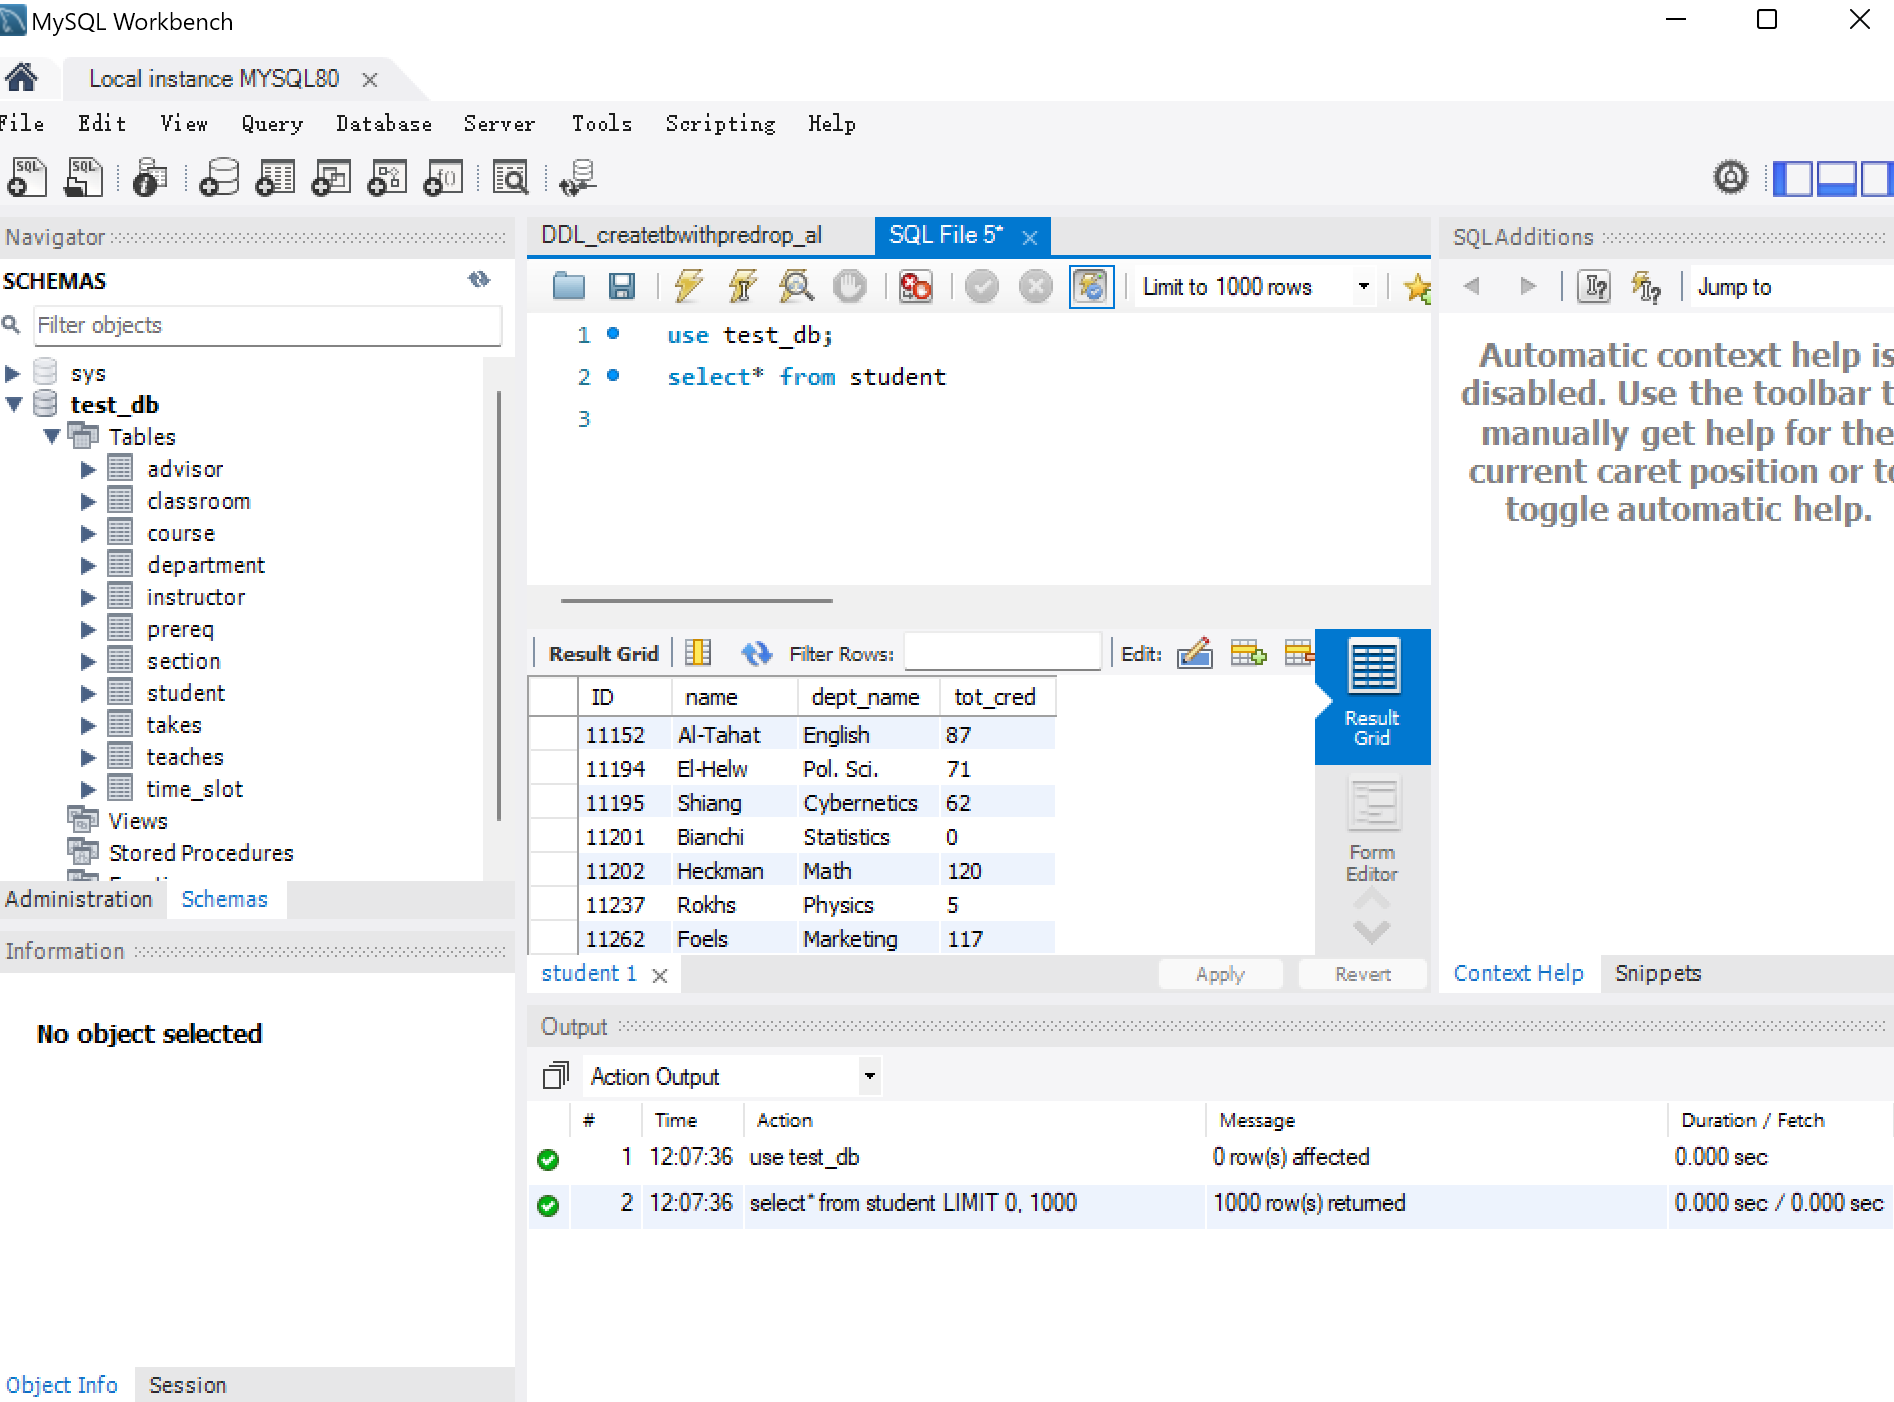
\includegraphics[width=12cm]{figure/数据截图1.png} \\
\footnotesize 图1 实验结果截图
\end{center}
\chapter{实验总结}
通过本次实验，我掌握了 MySQL 数据库的安装与配置方法，以及使用 MySQL Workbench 导入 SQL 文件数据的操作。在实验过程中，遇到了一些问题，例如 MySQL 安装时端口冲突、SQL 文件导入失败等，但通过查阅资料和调试，最终都得到了解决。这让我更加熟悉了 MySQL 数据库的使用，也提高了自己解决问题的能力。

\end{spacing}

\end{document}